\documentclass{ximera}
\input{../../preamble.tex}
\license{Creative Commons 3.0 By-NC}
\outcome{ Define a critical point.}
\outcome{ Find critical points.}
\outcome{ Define absolute maximum and absolute minimum.}
\outcome{ Find the absolute max or min of a continuous function on a closed interval.}
\outcome{ Define local maximum and local minimum.}
\outcome{ Compare and contrast local and absolute maxima and minima.}
\outcome{ Identify situations in which an absolute maximum or minimum is guaranteed.}
\outcome{ Classify critical points.}
\outcome{ State the First Derivative Test.}
\outcome{ Apply the First Derivative Test.}
\begin{document}

\begin{exercise}

	The graph of $y=f'(x)$ is below, for a function $f$.
	\begin{center}
		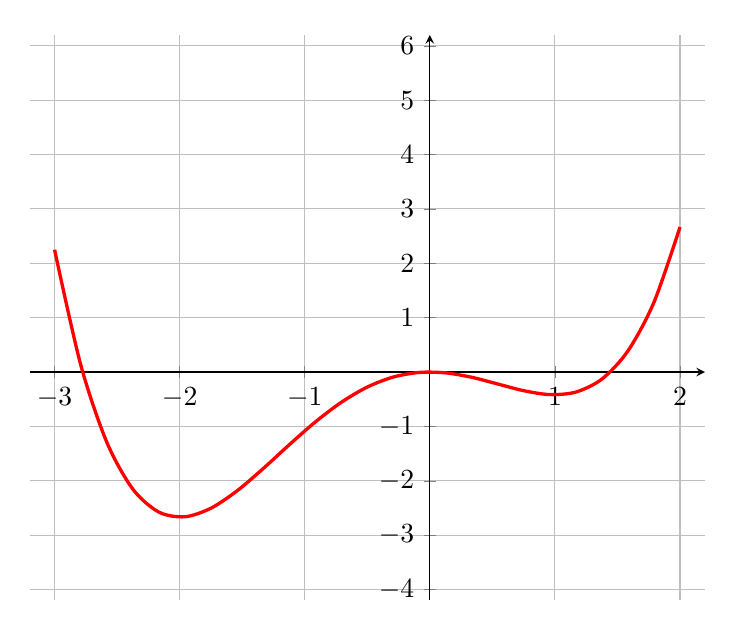
\begin{tikzpicture}[scale=1]
			\begin{axis}[
				xmin=-3.2, xmax=2.2, ymin=-4.2,ymax=6.2,    
				axis lines =middle, 
				every axis y label/.style={at=(current axis.above origin),anchor=south},
				every axis x label/.style={at=(current axis.right of origin),anchor=west},
				xtick={-3,...,2}, ytick={-4,..., 6},
				grid=major, width=4in,
				]
				\addplot[color=red, very thick, smooth, domain=-3:2]{0.25*x^4+(1/3)*x^3-x^2};
			\end{axis}
		\end{tikzpicture}
	\end{center}	

	On which intervals is $f$ concave up?
	\[ \left( \, \answer{-2} \, , \, \answer{0} \, \right) \,\, , \,\, \left( \, \answer{1} \, , \, \answer{\infty} \, \right) \]
	How many inflection points does $f$ have? $\answer{3}$.
	\begin{exercise}
		List the inflection points, from smallest to largest.
		\[ \answer{-2} \,\, , \,\, \answer{0} \,\, , \,\, \answer{1} \]
		\begin{exercise}
			The function $f$ has a critical point on the interval $(-3,-2)$.  
			That critical point is \wordChoice{ \choice[correct]{a local maximum}\choice{a local minimum}\choice{not a local extremum}}.
			
			The function $f$ has a critical point at $x=0$.
			That critical point is \wordChoice{ \choice{a local maximum}\choice{a local minimum}\choice[correct]{not a local extremum}}.

			The function $f$ has a critical point on the interval $(1,2)$.  
			That critical point is \wordChoice{ \choice{a local maximum}\choice[correct]{a local minimum}\choice{not a local extremum}}.
		\end{exercise}
	\end{exercise}
\end{exercise}
\end{document}
